%
% 00_Einleitung.tex
%
% (c) 2023 Florian Baumgartner, OST Ostschweizer Fachhochschule
%
% !TEX root = ../../buch.tex
% !TEX encoding = UTF-8
%
\section{Einleitung\label{autotune:section:teil0}}
\rhead{Einleitung}
Auto-Tune ist eine Technologie, die in der Musikindustrie zur Tonhöhenkorrektur von Gesang und instrumentalen Musikstücken verwendet wird.
Erfunden wurde Auto-Tune im Jahr 1997 von Dr. Andy Hildebrand, einem Erdölgeophysiker,
der seine Kenntnisse der digitaler Signalverarbeitung zur Erkundung von Erdölvorkommen nutzte,
um ein Werkzeug zur Korrektur musikalischer Tonhöhen zu schaffen.
Seine Erfindung, die unter dem Namen Auto-Tune bekannt wurde, hatte drastische Veränderungen in der Musikindustrie zur Folge.

Auto-Tune analysiert die Tonhöhen einer Aufnahme und passt sie so an, dass sie mit den für die Musik relevanten Tönen in Einklang gebracht werden,
in der Regel den Tönen einer diatonischen Tonleiter.
Dies kann verwendet werden, um falsche Töne zu korrigieren oder um künstlerische Effekte zu erzeugen, indem die Stimme stark moduliert wird.

Seit seiner Einführung hat sich Auto-Tune zu einem unverzichtbaren Werkzeug in der Musikproduktion entwickelt,
das in einer Vielzahl von Genres eingesetzt wird.
Es hat nicht nur die Art und Weise verändert, wie Musik aufgenommen und produziert wird,
sondern auch die Klanglandschaft der zeitgenössischen Musik geprägt.

Trotz der weitreichenden Anwendung und des Erfolgs von Auto-Tune bleibt die zugrunde liegende Technologie ein faszinierendes Thema der Signalverarbeitung.
Insbesondere die Beziehung zwischen Auto-Tune und der harmonischen Analysis ist ein reichhaltiges Forschungsfeld,
das immer noch eine Fülle von Entdeckungen und Entwicklungen zu bieten hat.


\subsection{Funktionsweise
\label{autotune:subsection:funktionsweise}}
Das Blockschaltbild in Abbildung \ref{autotune:fig:blockschaltbild} zeigt die grundlegende Funktionsweise von Auto-Tune.
Wichtig zu beachten ist, dass es sich hierbei um eine vereinfachte Darstellung handelt.
Kommerzelle Produkte basieren oft auf proprietären Algorithmen, welche nicht öffentlich zugänglich sind.
Da es nicht im Interesse der Hersteller ist, ihre Algorithmen zu veröffentlichen,
wird in dieser Arbeit nur die grundlegende Funktionsweise von Auto-Tune erklärt.

\begin{figure}
	\centering
	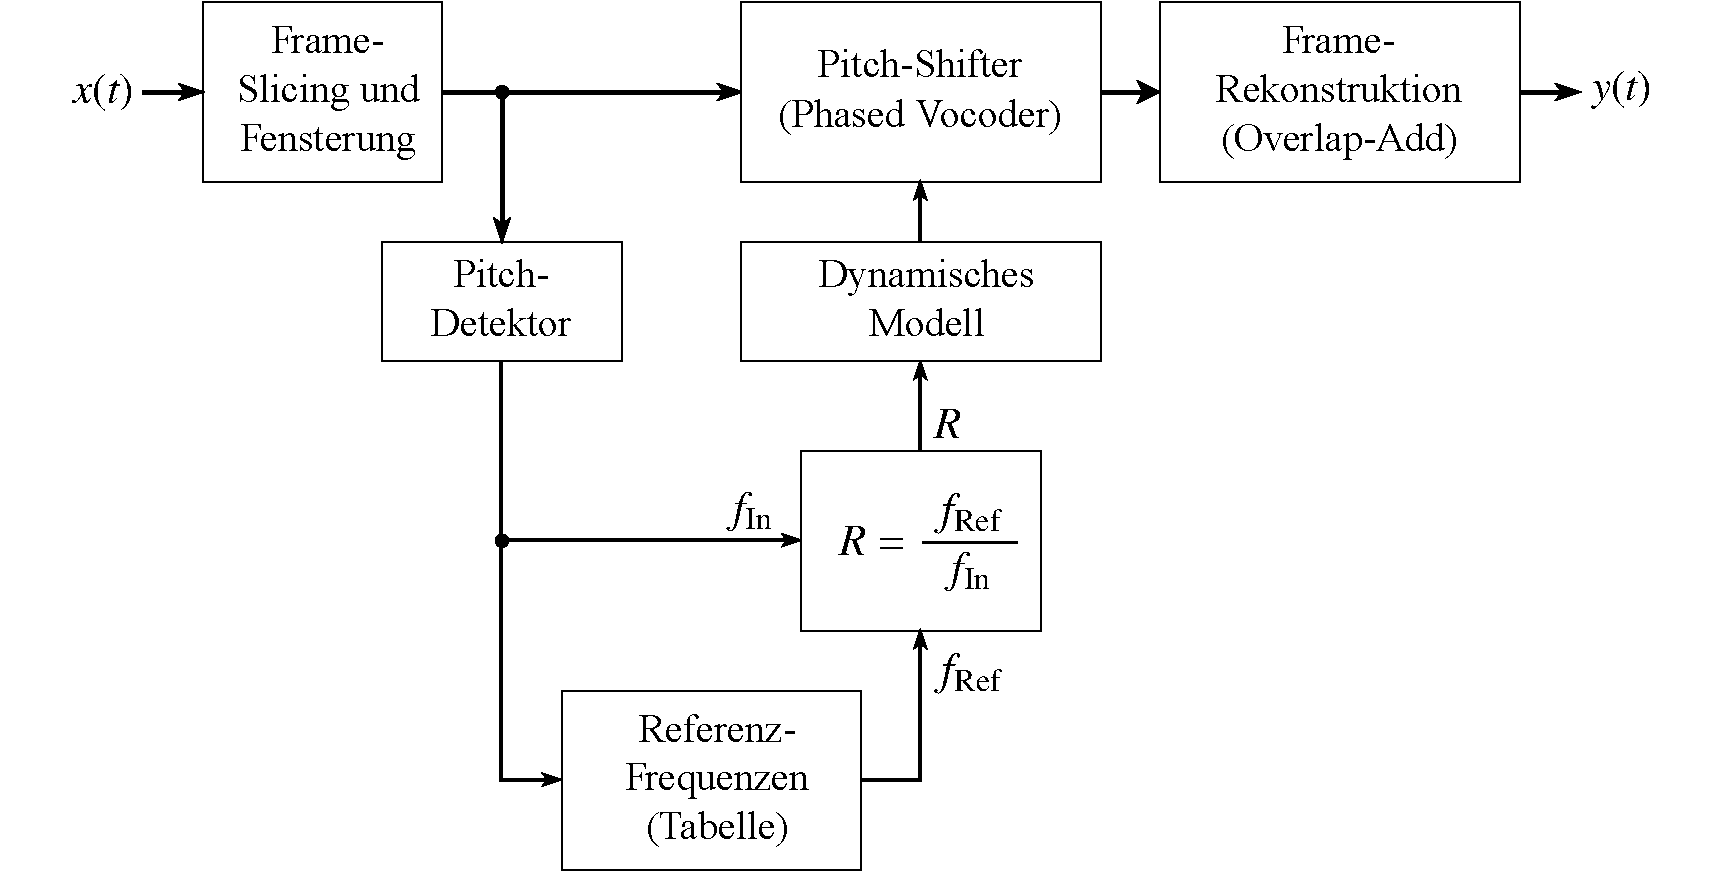
\includegraphics[width=\textwidth]{papers/autotune/images/Blockdiagram.pdf}
	\caption{Blockschaltbild von Auto-Tune Algorithmus.}
    \label{autotune:fig:blockschaltbild}
\end{figure}


\subsection{Signalfluss}
\label{autotune:subsection:signalfluss}
In der Praxis wird zwischen Real-Time und Non-Real-Time Auto-Tune unterschieden.
Bei Real-Time Auto-Tune wird das Signal in Echtzeit verarbeitet und die korrigierten Töne werden sofort ausgegeben.
Die maximale Latenzzeit darf dabei nicht mehr als 20\;ms betragen.
Dies ist nötig, damit die korrigierten Töne nicht als verzögert wahrgenommen werden.
Dadurch ist die Komplexität der Algorithmen beschränkt, weshalb diese oft im Zeitbereich arbeiten.

In dieser Arbeit liegt der Fokus auf Non-Real-Time Auto-Tune, das qualitativ wesentlich bessere Ergebnisse liefert.
Das generelle Konzept bleibt jedoch das Gleiche.

Um die Töne einer Melodie zu korrigieren, müssen zuerst die Tonhöhen der Einzeltöne erkannt werden.
Anschliessend werden diese verglichen mit einer Referenztonskala und die Abweichung wird entsprechend korrigiert.
Oftmals wird zusätzlich ein dynamisches Modell verwendet um Tonsprünge natürlicher klingen zu lassen.
Auf dieses wird in dieser Arbeit jedoch nicht eingegangen.

Kommerzielle Auto-Tune Produkte bieten oft noch weitere Funktionen wie z.B. die Tonhöhenkorrektur von mehrstimmigem Gesang oder das Anpassen der Formanten (siehe \ref{autotune:subsection:formantenErhaltung}).
